%\documentclass[aspectratio=10]{beamer} %For normal presentation (comment otherwise)
\documentclass[aspectratio=169]{beamer} %for widescreen prestentation
\usetheme{default}%{Singapore}
\usefonttheme{serif}
\usepackage{ulem}
\usecolortheme{default}%albatross, crane, beetle, dove, fly, seagull, wolverine e beaver.
\setbeamertemplate{frametitle}[default][center]
%%%%%%%%%%%%%%%%%%%%%%%%%%%%%%%%%%%%%%%%%%%%%%%%%%%%%%%%%%%%%%%%%%%%%%%%%%%%%%%%%%%%%%%%%%%%%%%
%%%%%%%%%%%%%%%%%%%%%%%%%%%%%%%%%%%%%%EXTRA PACTAGES%%%%%%%%%%%%%%%%%%%%%%%%%%%%%%%%%%%%%%%%%%%
\usepackage[utf8]{inputenc}
\usepackage[T1]{fontenc}
\usepackage[scaled]{helvet}
\renewcommand*\familydefault{\sfdefault}
\usepackage[portuguese, english]{babel}
\usepackage[round]{natbib}
\usepackage{hyperref} 
\usepackage{tcolorbox}
\usepackage{graphicx} % Required for including images
\usepackage{graphics}
%\usepackage[dvips]{graphicx} 
\graphicspath{{images/}} % Location of the graphics files
\usepackage{booktabs} % Top and bottom rules for table
\usepackage[font=small,labelfont=bf]{caption}%specifies captions on tables and figures
\usepackage{amsfonts, amsmath, amsthm, amssymb} % For math fonts, symbols and environments
\usepackage{wrapfig} % Allows wrapping text around tables and figures
\usepackage{makeidx}
\usepackage{epstopdf}%adiciona imagens em formato eps no pdf.
\usepackage{subfigure}%cria ambientes de multifiguras
\usepackage{float}%coloca as figuras exatamente aonde você quer
\usepackage{times}
\usepackage{tikz}%pacote para fazer fluxogramas
\usepackage{epsfig}
\usepackage{graphicx}
\usepackage{epstopdf} %converting to PDF
\usepackage{verbatim}%
\usepackage{multicol}
\usepackage{xcolor}
\usepackage[makeroom]{cancel}
\usepackage[framemethod=tikz]{mdframed}
\usepackage{hyperref} 
\usepackage{smartdiagram}
\usepackage{amssymb}
\usepackage{etoolbox}
\usepackage{multimedia}
\usepackage{media9}

%\smartdiagramset{uniform color list=gray!60!black for 6 items,
%back arrow disabled=false}
\usepackage{booktabs} % Top and bottom rules for table
\usepackage[font=small,labelfont=bf]{caption} % Required for specifying captions to 

%%%%%%%%%%%%%%%%%%%%%%%%%%%%%%%%%%%%%%%%%%%%%%%%%%%%%%%%%%%%%%%%%%%%%%%%%%%%%%%%%%%%%%%%%%%%%
%%%%%%%%%%%%%%%%%%%%%%%%%%%%%%%%%%%%% PREAMBLE %%%%%%%%%%%%%%%%%%%%%%%%%%%%%%%%%%%%%%%%%%%%%%%%
%\subtitle{}
\author[Seu nome aqui]{Nome Sobrenome} 
\title{Título da sua apresentação}
\subtitle{Projeto PR4}
\date{mês e ano}
\subject{}
%\setbeamertemplate{footline}[frame number]
%\setbeamercovered{transparent}
\setbeamertemplate{navigation symbols}{}
% Tela cheia
\hypersetup{pdfpagemode=FullScreen}
\usepackage{ragged2e}
%\justifying
%\addtobeamertemplate{headline}{}
\usepackage{tikz}
\usetikzlibrary{shapes.geometric, arrows}

% Criar um novo comando para destacar o primeiro item
\patchcmd{\sectioninToC}{\inserttocsection}{\ifnumequal{\inserttocsectionnumber}{1}{\textbf{\inserttocsection}}{\inserttocsection}}{}{}


%%%%%%%%%%%%%%%%%%%%%%%%%%%%%%%%%%%%%%%%%%%%%% PRESENTATION %%%%%%%%%%%%%%%%%%%%%%%%%%%%%%%%%%%%%%%%%%%%%%%
\begin{document}


\bgroup
\makeatletter
\setbeamertemplate{footline}
\makeatother
%\maketitle
\egroup
\scriptsize 
\addtobeamertemplate{navigation symbols}{}{\hskip6pt\raisebox{2pt}{\color{blue}\insertframenumber}}
\setcounter{framenumber}{0}
%\AtBeginSection[]



%%% CAPA
{
\usebackgroundtemplate{
\centering

\includegraphics[width=\paperwidth,height=\paperheight]{images/capa.jpg}% Você pode escolher mudar a capa para o modelo antigo aqui!!!!!
}
	
% Frame 3: plano de fundo
\begin{frame}

	
\end{frame}
}


%% TÍTULO

{
\usebackgroundtemplate{
\centering

\includegraphics[width=\paperwidth,height=\paperheight]{images/base.png} %imagem de fundo padrão
}
	

\begin{frame}
\maketitle
	
\end{frame}
}




\section{Pauta da reunião (Seção 1)}
\section{Pauta da reunião (Seção 2)}
\section{Pauta da reunião (Seção 3)}






{
\usebackgroundtemplate{
\centering
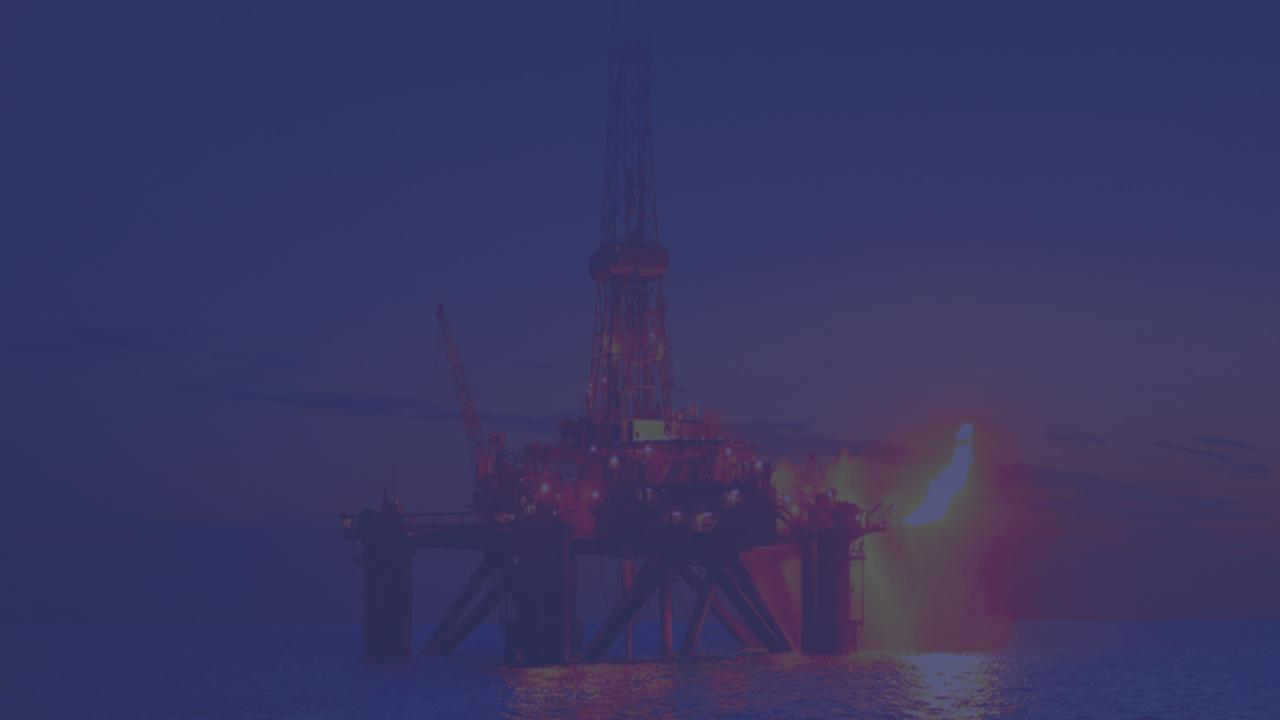
\includegraphics[width=\paperwidth,height=\paperheight]{images/fundonovo.jpg}
}

\begin{frame}
	\centering
	\frametitle{\textcolor{white}{Pauta}}
    %\large
	\setbeamercolor{section in toc}{fg=white,bg=white}
    \tableofcontents[currentsection,sectionstyle=show/shaded,subsectionstyle=show/show/shaded]
\end{frame}

}


{
\usebackgroundtemplate{
\centering
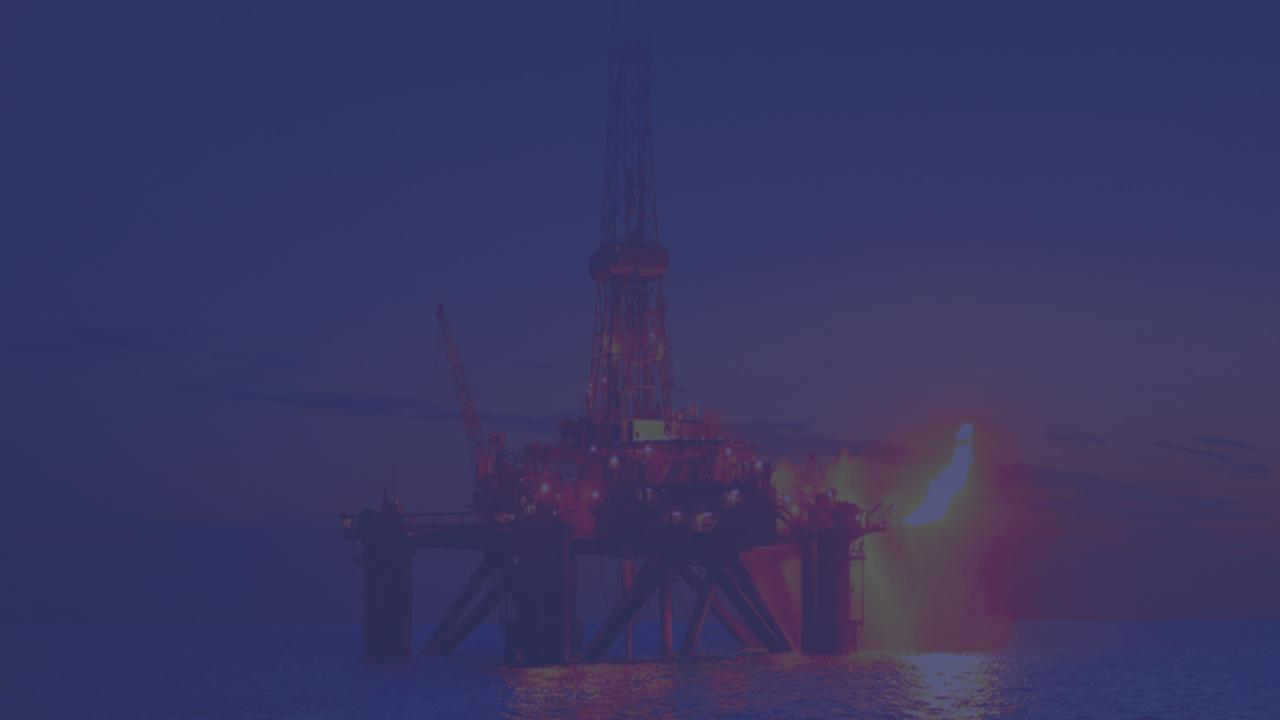
\includegraphics[width=\paperwidth,height=\paperheight]{images/fundonovo.jpg}
}
\begin{frame}
\vspace{1cm}
\begin{center}
\huge
\textcolor{orange}{Pauta da reunião (Seção 1)}
\end{center}

\end{frame} 
}



{
\usebackgroundtemplate{
\centering

\includegraphics[width=\paperwidth,height=\paperheight]{images/base.png}
}

{ \begin{frame}
\frametitle{Escreva aqui o título do slide}

	Local para escrever algo ...


	\begin{figure}
		\centering
		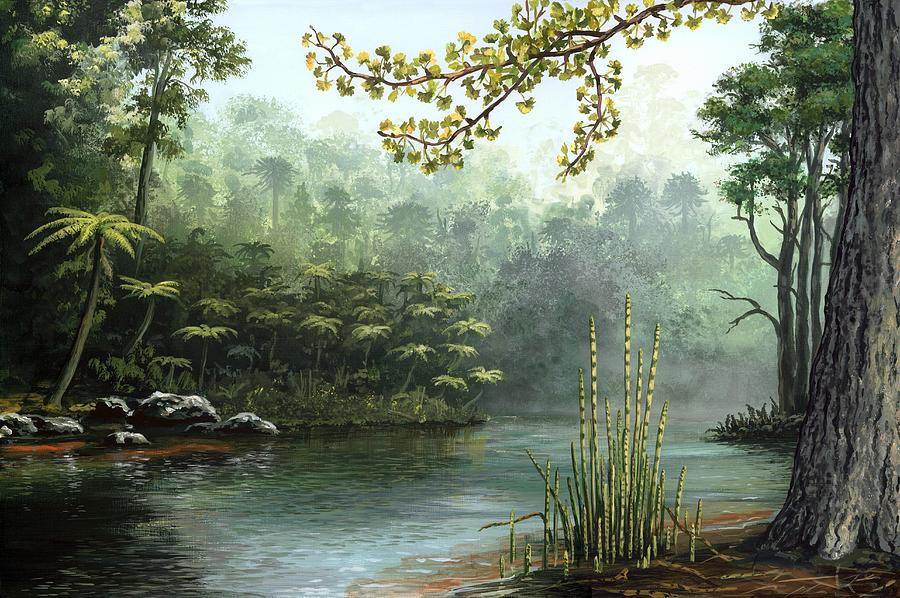
\includegraphics[scale=0.7]{images/jur.jpg}
		\caption{Fale sobre a figura e inclua uma referência \cite{thomas2022}}
	\end{figure}

\begin{flushleft}
    \begin{columns}

    \column{0.5\textwidth}
        \centering

     \begin{itemize}
	     \pause
	     \item observação 1
	     \pause
	     \item observação 2
     \end{itemize}    
    
  % \column{0.01\textwidth}
                               
    \end{columns}

\end{flushleft}


\end{frame} 
} 






{
\usebackgroundtemplate{
\centering
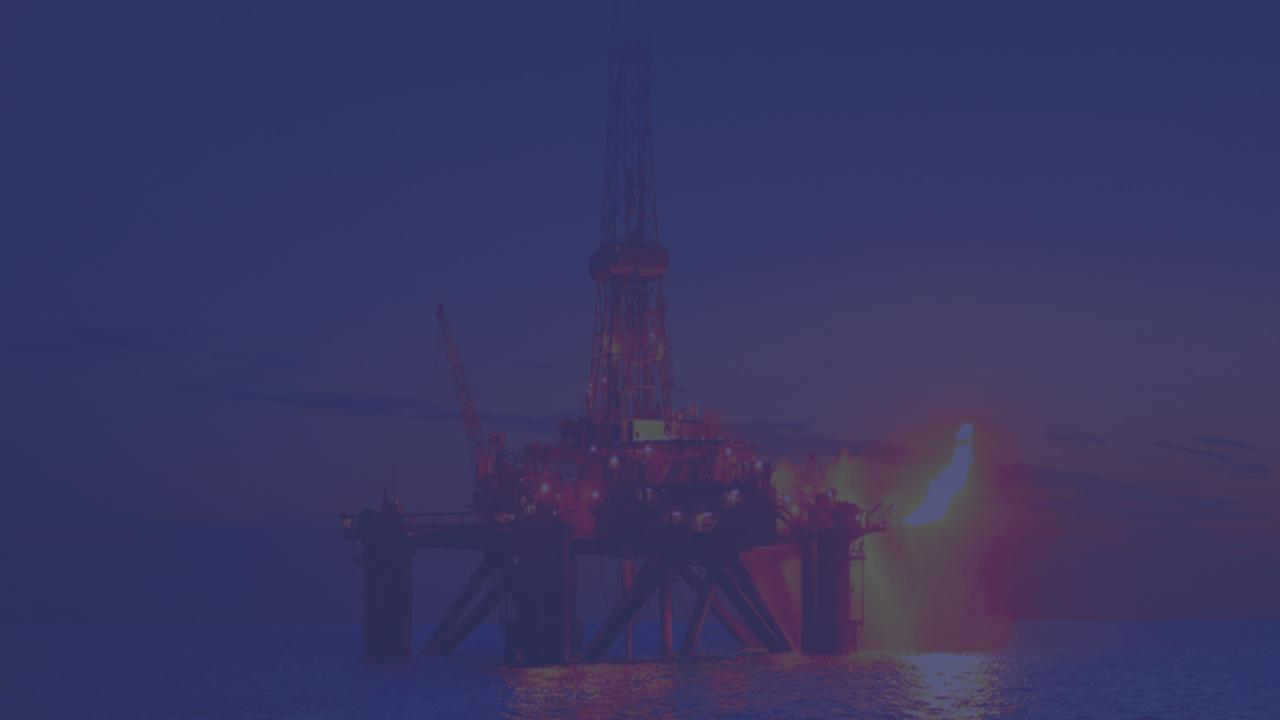
\includegraphics[width=\paperwidth,height=\paperheight]{images/fundonovo.jpg}
}
\begin{frame}
\vspace{1cm}
\begin{center}
\huge
\textcolor{orange}{Pauta da reunião (Seção 2)}
\end{center}

\end{frame} 
}







{
\usebackgroundtemplate{
\centering

\includegraphics[width=\paperwidth,height=\paperheight]{images/base.png}
}
\begin{frame}	
\frametitle{Título}
%	\begin{figure}
%		\centering
%		\includegraphics[scale=0.3]{images/pipelineachillesia.png}
%		\caption{A biblioteca consiste em dependências somadas aos módulos de treino e predição.}
%	\end{figure}


\end{frame}
}




{
\usebackgroundtemplate{
\centering

\includegraphics[width=\paperwidth,height=\paperheight]{images/base.png}
}
\begin{frame}	
\frametitle{Título}

%\movie[width=0.8\linewidth,height=0.6\linewidth,showcontrols]{Clique para reproduzir}{images/frontend.mp4}


\begin{center}
    \footnotesize
\includemedia[
    width=0.8\linewidth,
    height=0.5\linewidth,
    activate=onclick,
    addresource=frontend.mp4,
    addresource=images/achillesia_logo.png,
    flashvars={
        source=frontend.mp4
        &autoPlay=false
        &poster=images/achillesia_logo.png
        &playbutton=images/playbutton.png
    }
]{}{frontend.mp4}

\end{center}



\end{frame}
}





%%%%%%%%%%%%%%%%%%%%%%%%%%%%%%%%%%%%%%% REFERENCES %%%%%%%%%%%%%%%%%%%%%%%%%%%%%%%%%%%%%%%%%%%%%%%%%


{
\usebackgroundtemplate{
\centering

\includegraphics[width=\paperwidth,height=\paperheight]{images/base.png}
}
\begin{frame}[allowframebreaks]
\frametitle{Referências}
\beamertemplatetextbibitems
\tiny
\bibliographystyle{apalike}
\bibliography{refs}
\end{frame}
}



\makeatother

{
\usebackgroundtemplate{
\centering

\includegraphics[width=\paperwidth,height=\paperheight]{images/interlocucao.png}
}
	
% Frame 3: plano de fundo
\begin{frame}

	
\end{frame}
}

{
\usebackgroundtemplate{
\centering

\includegraphics[width=\paperwidth,height=\paperheight]{images/agradecimento.png}
}
	
% Frame 3: plano de fundo
\begin{frame}





\end{frame}
}
\end{document}
